%------------------------------------------------------------------------------
% Template file for the submission of papers to IUCr journals in LaTeX2e
% using the iucr document class
% Copyright 1999-2013 International Union of Crystallography
% Version 1.6 (28 March 2013)
%------------------------------------------------------------------------------


\documentclass[preprint]{iucr}              % DO NOT DELETE THIS LINE
\usepackage{amssymb}
\usepackage[fleqn]{amsmath}
%\usepackage{bm}
\usepackage{graphicx}
\usepackage{tabularx}
\usepackage{booktabs}
%\usepackage{calligra}
\usepackage{array}
\DeclareMathAlphabet{\mathcalligra}{T1}{calligra}{m}{n}
\def\mathbi#1{\textbf{\em #1}}
\numberwithin{equation}{section}
%\DeclareMathSymbol{\Gamma}{\mathalpha}{letters}{"00}
%\DeclareMathSymbol{\Lambda}{\mathalpha}{letters}{"03}
%\DeclareMathSymbol{\Omega}{\mathalpha}{letters}{"0A}
%\DeclareMathAlphabet{\mathitbf}{OML}{cmm}{b}{it}
\hyphenation{Niggli}
\def\mathbi#1{\textbf{\em #1}}
%\numberwithin{equation}{section}
%\DeclareMathSymbol{\Gamma}{\mathalpha}{letters}{"00}
%\DeclareMathSymbol{\Lambda}{\mathalpha}{letters}{"03}
%\DeclareMathSymbol{\Omega}{\mathalpha}{letters}{"0A}
%\DeclareMathAlphabet{\mathitbf}{OML}{cmm}{b}{it}
\usepackage{color}
%\usepackage{ulem}
\usepackage{url}
\usepackage{yfonts}
%\usepackage{xr-hyper}
%\usepackage[draft]{hyperref}
%\usepackage{bibentry}
\usepackage[normalem]{ulem}
\usepackage{listings}

% Redefine \underline to use \textit
\renewcommand{\underline}[1]{\textit{#1}}

% Crystallographic space macros
\newcommand{\HVI}{\ensuremath{\mathbf{H}^{6}}}
\newcommand{\GVI}{\ensuremath{\mathbf{G}^{6}}}
\newcommand{\SVI}{\ensuremath{\mathbf{S}^{6}}}
\newcommand{\PIII}{\ensuremath{\mathbf{P}^{3}}}
\newcommand{\FIII}{\ensuremath{\mathbf{F}^{3}}}
\newcommand{\CIII}{\ensuremath{\mathbf{C}^{3}}}
\newcommand{\RIII}{\ensuremath{\mathbb{R}^{3}}}

\newcommand{\vdotv}[2]{${{\bf #1 \cdot #2}}$}
\newcommand{\Imaginary}[0]{\mathcal{I}}
\newcommand{\Real}[0]{\mathcal{R}}
\newcommand{\Exchange}[0]{$\mathcal{X}$}

\newcommand{\nounderline}[3]{\!\!\!\!\!\!\!\!\!#1,&\!\!\!\!\!\!\!\!\!#2,&\!\!\!\!\!\!\!\!\!#3}
\newcommand{\underlineab}[3]{\!\!\!\!\!\!\!\!\!\!\!\!\!\!\!\!\!\!\!\!\!\!\!\!\Exchange{}(#1),&\!\!\!\!\!\!\!\!\!\!\!\!\!\!\!\!\!\!\!\!\!\!\!\!\Exchange{}(#2),&\!\!\!\!\!\!\!\!\!#3}
\newcommand{\underlineac}[3]{\!\!\!\!\!\!\!\!\!\!\!\!\!\!\!\!\!\!\!\!\!\!\!\!\Exchange{}(#1),&\!\!\!\!\!\!\!\!\!\!\!\!\!\!\!\!\!\!\!\!\!\!\!\!#2,&\!\!\!\!\!\!\!\!\!\Exchange{}(#3)}
\newcommand{\underlinebc}[3]{\!\!\!\!\!\!\!\!\!\!\!\!\!\!\!\!\!\!\!\!\!\!\!\!#1,&\!\!\!\!\!\!\!\!\!\Exchange{}(#2),&\!\!\!\!\!\!\!\!\!\!\!\!\!\!\!\!\!\!\!\!\!\!\!\!\Exchange{}(#3)}

\newcommand{\scalar}[1]{$#1$}

\newcommand{\scalarsub}[2]{$#1_#2$}

%-------------------------------------------------------------------------
% Information about journal to which submitted
%-------------------------------------------------------------------------
\journalcode{A}              % Indicate the journal to which submitted
%   A - Acta Crystallographica Section A
%   B - Acta Crystallographica Section B
%   C - Acta Crystallographica Section C
%   D - Acta Crystallographica Section D
%   E - Acta Crystallographica Section E
%   F - Acta Crystallographica Section F
%   J - Journal of Applied Crystallography
%   M - IUCrJ
%   S - Journal of Synchrotron Radiation
\makeatletter
\font\dummyft@=dummy \relax
\makeatother

\begin{document}                  % DO NOT DELETE THIS LINE
	
	%-------------------------------------------------------------------------
	% The introductory (header) part of the paper
	%-------------------------------------------------------------------------
	
	% The title of the paper. Use \shorttitle to indicate an abbreviated title
	% for use in running heads (you will need to uncomment it).
	
	% Authors' names and addresses. Use \cauthor for the main (contact) author.
	% Use \author for all other authors. Use \aff for authors' affiliations.
	% Use lower-case letters in square brackets to link authors to their
	% affiliations; if there is only one affiliation address, remove the [a].
	
	% Use \vita if required to give biographical details (for authors of
	% invited review papers only). Uncomment it.
	
	% lca IUCr id IUCr6401
	%\vita{Author's biography}
	
	% Keywords (required for Journal of Synchrotron Radiation only)
	% Use the \keyword macro for each word or phrase, e.g. 
	% \keyword{X-ray diffraction}\keyword{muscle}
	
	
	% PDB and NDB reference codes for structures referenced in the article and
	% deposited with the Protein Data Bank and Nucleic Acids Database (Acta
	% Crystallographica Section D). Repeat for each separate structure e.g
	% \PDBref[dethiobiotin synthetase]{1byi} \NDBref[d(G$_4$CGC$_4$)]{ad0002}
	
	%\PDBref[optional name]{refcode}
	%\NDBref[optional name]{refcode}
	
	%-------------------------------------------------------------------------
	% The introductory (header) part of the paper
	%-------------------------------------------------------------------------
	
	% The title of the paper. Use \shorttitle to indicate an abbreviated title
	% for use in running heads (you will need to uncomment it).
	\begin{center}
	{\LARGE \emph{\today}} \\
\end{center}

\title{Approximate Supercell (Superlattice) Matching}
\shorttitle{3D Supercell Matching}

% Authors' names and addresses. Use \cauthor for the main (contact) author.
% Use \author for all other authors. Use \aff for authors' affiliations.
% Use lower-case letters in square brackets to link authors to their
% affiliations; if there is only one affiliation address, remove the [a].


\cauthor[a]{Lawrence C.}{Andrews}{larry6640995@gmail.com}{}
\author[b]{Herbert J.}{Bernstein}

\aff[a]{Ronin Institute for Independent Scholarship 2.0, USA}
\aff[b] {Fresh Pond Research Institute, Cambridge, Mass., USA}


% Use \shortauthor to indicate an abbreviated author list for use in
% running heads (you will need to uncomment it).


	% lca IUCr id IUCr6401
	% HJB IUCr id IUCr6484
	% NKS IUCr ID: IUCr7572
	% lca ORCID  0000-0002-4451-1641
	% HJB ORCID 0000-0002-0517-8532
	% NKS ORCID 0000-0003-2786-6552
	% Use \shortauthor to indicate an abbreviated author list for use in
	% running heads (you will need to uncomment it).
	% Use \vita if required to give biographical details (for authors of
	% invited review papers only). Uncomment it.
	
	% lca IUCr id IUCr6401
	%\vita{Author's biography}
	
	% Keywords (required for Journal of Synchrotron Radiation only)
	% Use the \keyword macro for each word or phrase, e.g. 
	% \keyword{X-ray diffraction}\keyword{muscle}
	
	\keyword{lattice}
	\keyword{reduction}
	\keyword{SuperCell}
	\keyword{matching}
	
	% PDB and NDB reference codes for structures referenced in the article and
	% deposited with the Protein Data Bank and Nucleic Acids Database (Acta
	% Crystallographica Section D). Repeat for each separate structure e.g
	% \PDBref[dethiobiotin synthetase]{1byi} \NDBref[d(G$_4$CGC$_4$)]{ad0002}
	
	%\PDBref[optional name]{refcode}
	%\NDBref[optional name]{refcode}
	
	\maketitle                        % DO NOT DELETE THIS LINE
	
	\newcommand{\OPES}[0]{$E^3toS^6$}
	\newcommand{\OPESS}[0]{$$E^3toS^6$$}
	\newcommand{\MSVI}[0]{$M_{S^{6}}$}
	\newcommand{\MEIII}[0]{$M_{E^{3}}$}
	\newcommand{\Plus}[0]{\mathcal{P}}	
	\newcommand{\Minus}[0]{\mathcal{M}}
	
	\newcommand{\ci}[0]{$c_1$}
	\newcommand{\cii}[0]{$c_2$}
	\newcommand{\ciii}[0]{$c_3$}
	
	
	\begin{abstract}
A solution is presented for determining the relationship between two unit cells when one is a supercell of the other.
	\end{abstract}
	% Appendices appear after the main body of the text. They are prefixed by
	% a single \appendix declaration, and are then structured just like the
	% body text.
	
\vspace{4mm}
\hfill\begin{minipage}{0.62\linewidth}
	\itshape\small
	Siblings are recognized at a glance, cousins on reflection, and
	ancestors only by argument. An acquaintance may be mistaken for
	any of them.
	\vspace{1mm}
	
	\upshape\normalfont\raggedleft
	--- Claude (Anthropic), 2026
\end{minipage}
\vspace{4mm}


\section{Synopsis}
A solution is proposed for the problem of best matching of a unit cell to a supercell.


	
	\section{Introduction}

\citeasnoun{santoro1980determination} enumerated transformation 
{matrices} for generating coincidence site lattices (superlattices)
from a given unit cell description. They create one exact representation
of a superlattice for each choice of input and transformation. The
general solution requires awareness of different choices of unit cells, 
alternative choices for basis vectors for actual or near degeneracies,
and allowance for lattice distortion (for instance, because of
replacement on one metal ion with another).
	
	\citeasnoun{andrews2026approximate} describe a general solution for finding 
	approximate relationships between unit cells that are similar but
	not necessarily sampled from the identically-same lattice.
	A user of that software (CmdLMP3) asked if the same could be applied to
	the determination of unit cells to supercells. Here we extend their method to the case of supercells.


\begin{figure}
	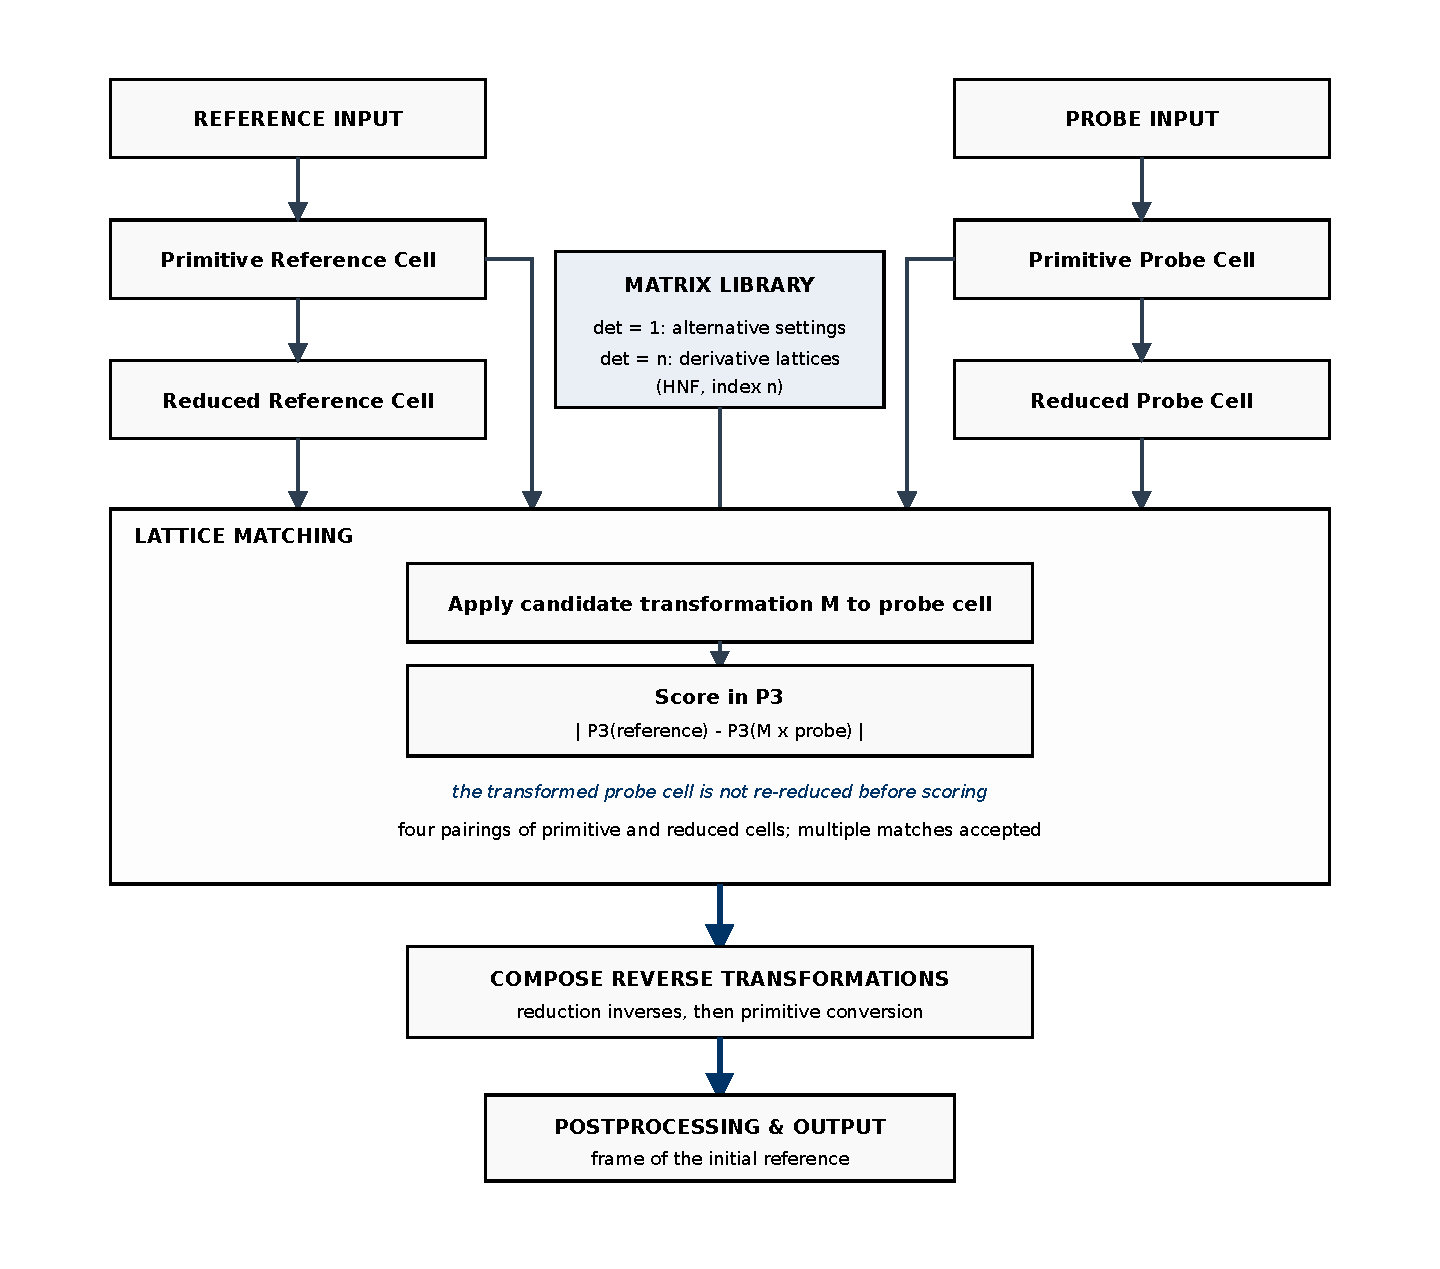
\includegraphics[width=\columnwidth]{supercell1}
	\label{process}
	\caption{The process of Andrews \& Bernstein (2026) for approximate matching of lattices.
		 Reference and probe cells are converted to primitive form and reduced. Both 
		 the primitive and the reduced cell of each are passed to the matching stage, 
		 giving four pairings. A library of matrices supplies candidate transformations 
		 of the probe: matrices of determinant one enumerate alternative settings of  
		 the probe lattice, and matrices of determinant n enumerate the derivative 
		 lattices of index n. Each candidate transformation is applied to the probe lattice and 
		 scored by the \PIII{} distance to the reference. The transformed cell 
		 is not reduced again before scoring, so the score depends on the setting 
		 as well as on the lattice. Accepted matches are carried back through 
		 the reduction and primitive-conversion inverses to the frame of 
		 the initial reference.
}
\end{figure}

\section{Algorithm}

The above algorithm suffices for matching lattices that are somewhat
similar to each other, but the question of matching a cell to a supercell
can be tackled with a modest modification. Where matching above is
done using unimodular matrices, by replacing the library of transformation
matrices with a library  of matrices that have larger determinants, approximate
supercell relationships can be determined.

For instance, for a given unit cell, to find supercells that have 
a base vector tripled a library of transformations with 
determinant=3.0 would be used. Other than that, the algorithm 
would only need output reporting changed.
	
	\section{Notation}
	
\noindent \PIII{}: Polar coordinate space is a compact and smooth alternative to lengths and angles. \PIII{} is useful for comparing unit cells. \cite{andrews2026p3}
	\PIII{}: 
		$(|\vec{a}|,\alpha),\ (|\vec{b}|,\beta),\ (|\vec{c}|,\gamma)$\\
	$\Rightarrow$\\
	\hspace*{0.5cm}$(|\vec{a}|\cos\alpha,\, |\vec{a}|\sin\alpha)$\\
	\hspace*{0.5cm}$(|\vec{b}|\cos\beta,\, |\vec{b}|\sin\beta)$\\
	\hspace*{0.5cm}$(|\vec{c}|\cos\gamma,\, |\vec{c}|\sin\gamma)$\\
	also known as $(p_1, p_2, p_3)$


\section{Implementation details}

\subsection{Matrix generator}
Appendix \ref{generator} is a $C^{++}$ function for generating
libraries of matrices with specified integer valued determinants. In program CmdLMP3, this function is used
to create the library of matrices that are used for
approximate lattice matching.

\subsection{Determinants}

	For each value of determinants (n), the number of possible
	matrices with maximum elements (-n,n), the number of 
	possible matrices grows rapidly. See Table \ref{tab:matrix_determinants}.
	
% Requires no packages beyond standard LaTeX.
% If the journal style is two-column, change table to table*.

% Requires no packages beyond standard LaTeX.
% If the journal style is two-column, change table to table*.

\begin{table}
		\label{tab:matrix_determinants}
	\caption{Transformation matrix counts by determinant class. For $n=1$ and $n=2$
		the complete set is used in CmdLMP3. For $n=3$ and $n=4$ the complete set is used with the
		13 and 35 Hermite normal forms appended, respectively; those matrices are already present in
		the complete set, so the appended copies are redundant and are retained only as
		a guard. For index $n=5$ and index $n=6$ the exhaustive search is not attempted, as it would
		screen $2.4\times10^{9}$ and $1.1\times10^{10}$ candidates to yield sets of
		$1.4\times10^{7}$ and $7.1\times10^{7}$ matrices. In their place the 3480
		matrices of determinant one are composed with the Hermite normal forms of index
		5 and 6 in both right and left multiplication orders. Left multiplication preserves the lattice
		and supplies alternative settings of it; right multiplication changes the
		lattice. The resulting sets span all 31 and all 91 derivative lattices, but
		sample the settings of each lattice less densely than the exhaustive sets at lower index.}
		
	\label{tab:matrixcounts}
	
	\vspace{2mm}
	
	\begin{tabular}{crrrr}
		\hline
		& Derivative       & Candidates          & Complete       & Used in \\
		$n$   & lattices\dag     & screened\ddag       & set\S          & CmdLMP3\P \\
		\hline
		1     &  1 &         19\,683 &        3\,480 &       3\,480 \\
		2     &  7 &   1\,953\,125 &    147\,696 &     147\,696 \\
		3     & 13 &  40\,353\,607 & 1\,060\,920 &  1\,060\,933 \\
		4     & 35 & 387\,420\,489 & 6\,721\,896 &  6\,721\,931 \\
		5     & 31 & 2\,357\,947\,691 & 13\,942\,248 &  215\,760 \\
		6     & 91 & 10\,604\,499\,373 & 70\,632\,144 &  633\,360 \\
		\hline
		Total & 177 & & 92\,508\,384 & 8\,783\,160 \\
		\hline
	\end{tabular}
	
	\vspace{2mm}
	
	\noindent
	{\dag} Number of distinct sublattices of index $n$ in a three-dimensional
	lattice. Each has exactly one Hermite normal form. The total excludes the
	trivial lattice at $n=1$.
	
	\noindent
	{\ddag} Size of the exhaustive search over integer matrices with coefficients in
	$[-n,n]$, the smallest symmetric box that contains every Hermite normal form of
	index $n$. Screening costs are not additive across independent searches, so no
	total is given.
	
	\noindent
	{\S} Number of those candidates having determinant $+n$. Matrices of negative
	determinant are excluded because they invert chirality.
	
	\noindent
	{\P} Number of matrices actually retained by CmdLMP3.
	
\end{table}


% ---------------------------------------------------------------------------
% Alternative, if footnote markers are unwanted: keep the column names in the
% caption but set them in italic rather than bold. Italic in caption prose
% carries less risk of being read as notation than bold, which IUCr reserves
% for vectors.
%
%   \emph{Derivative lattices} is the number of distinct sublattices ...
%   \emph{Candidates screened} is the size of the exhaustive search ...
%   \emph{Complete set} is the number of those candidates with determinant $+n$ ...
%   \emph{Used in CmdLMP3} is the number actually retained.
% ---------------------------------------------------------------------------

\subsection{Reference vs. probe decision}

For a given input pair of unit cells, the decision to 
search for supercells of the reference cell requires
that the reference have the smaller primitive unit
volume of the pair. The output of the results of matching
shows the transformation from the input probe cell to
the frame of the input reference cells. That might be
the reverse of the choice that the user desires, so
 the inverse 3x3 matrix is also output.



	



	


	\section{Examples}
	
	\subsection{Example 1}
{
\begin{verbatim}
=== TEST: Hawaiian ===
Description: Nearly identical cells with known transformation
Input cells:
Cell 1 (P):    10.250    10.740    21.080    87.720    75.970    61.530 
Cell 2 (P):    10.250    10.740    21.080    78.960    75.970    61.490 
; primitive cell volume ratio, mobile/reference
;  ratio = 1.000
; Found 403 results

; === LATTICE MATCHING RESULTS ===

; --- Match 1 ---
; EQUIVALENT  P3 distance: 0.010 (0.0% of P3 norm)  S6 angle: 0.01 deg
; Matrix:  [-1 0 0   -1 1 0   0 0 -1] (Determinant: 1.000)
; Inverse: [-1 0 0   -1 1 0   0 0 -1]
; P    10.250    10.740    21.080    87.720    75.970    61.530  [REFERENCE]
; P    10.250    10.739    21.080    87.714    75.970    61.502  [TRANSFORMED MOBILE (CONVENTIONAL)]

; --- Match 2 ---
; EQUIVALENT  P3 distance: 0.023 (0.1% of P3 norm)  S6 angle: 0.03 deg
; Matrix:  [-1 0 0   0 -1 0   -1 0 1] (Determinant: 1.000)
; Inverse: [-1 0 0   0 -1 0   -1 0 1]
; P    10.250    10.740    21.080    87.720    75.970    61.530  [REFERENCE]
; P    10.250    10.740    21.087    87.674    75.893    61.490  [TRANSFORMED MOBILE (CONVENTIONAL)]

\end{verbatim}

\subsection{Example 2}
\begin{verbatim}
	=== TEST: FaceDiagonalOrder2 ===
	Description: [SUPERCELL] Cubic doubled along face diagonal -- order-2, dist=0
	Input cells:
	Cell 1 (P):    10.000    10.000    10.000    90.000    90.000    90.000 
	Cell 2 (P):    14.142    14.142    10.000    90.000    90.000    90.000 
	; primitive cell volume ratio, mobile/reference
	;  ratio = 2.000   swapped reference and probe cells
	; Found 324 results
	
	; === LATTICE MATCHING RESULTS ===
	; === SUPERCELL ===  prim. cell volume ratio = 2.000
	
	; --- Match 1 ---
	; order-2 supercell  EXCELLENT  P3 distance: 0.000 (0.0% of P3 norm)  S6 angle: 0.00 deg
	; Matrix:  [1 -1 0   1 1 0   0 0 1] (Determinant: 2.000  [SUPERCELL])
	; Inverse: [1/2 1/2 0   -1/2 1/2 0   0 0 1]
	; P    14.142    14.142    10.000    90.000    90.000    90.000  [REFERENCE]
	; P    14.142    14.142    10.000    90.000    90.000    90.000  [TRANSFORMED MOBILE (CONVENTIONAL)]
	
	; --- Match 2 ---
	; order-2 supercell  EXCELLENT  P3 distance: 0.000 (0.0% of P3 norm)  S6 angle: 0.00 deg
	; Matrix:  [1 1 0   -1 1 0   0 0 1] (Determinant: 2.000  [SUPERCELL])
	; Inverse: [1/2 -1/2 0   1/2 1/2 0   0 0 1]
	; P    14.142    14.142    10.000    90.000    90.000    90.000  [REFERENCE]
	; P    14.142    14.142    10.000    90.000    90.000    90.000  [TRANSFORMED MOBILE (CONVENTIONAL)]
	
\end{verbatim}

\subsection{Example 3}

\begin{verbatim}
	=== TEST: Simon Parsons ===
	Description: [SUPERCELL] R primitive vs P triclinic -- order-4, dist=0.820
	Input cells:
	Cell 1 (P):     9.477     9.477     9.477    64.240    64.240    64.240 
	Cell 2 (P):     9.482    13.705    20.048    89.510    88.720    86.960 
	; primitive cell volume ratio, mobile/reference
	;  ratio = 3.953  swapped reference and probe cells
	; Found 300 results
	
	; === LATTICE MATCHING RESULTS ===
	; === SUPERCELL ===  prim. cell volume ratio = 4.000
	
	; --- Match 1 ---
	; order-4 supercell  POOR  P3 distance: 0.820 (3.1% of P3 norm)  S6 angle: 1.16 deg
	; Matrix:  [0 1 0   -1 1 -1   -2 0 2] (Determinant: 4.000  [SUPERCELL])
	; Inverse: [1/2 -1/2 -1/4   1 0 0   1/2 -1/2 1/4]
	; NOTE: P3 distance (3.146% of P3 norm) exceeds threshold 2.000% -- match is distorted
	; P     9.482    13.705    20.048    89.510    88.720    86.960  [REFERENCE]
	; P     9.477    13.834    20.155    90.000    90.000    84.859  [TRANSFORMED MOBILE]
	
	Validating using quality thresholds:
	Checking result 1 ([SUPERCELL] order-4 det~4 dist~1.9):
\end{verbatim}


	\section{Summary}
A method for determining whether  a reference cell and a probe cell have a subcell/supercell relationship and
for determining the three-dimensional
transformation matrices between them is described.

The described algorithm (CmdLMP3) on a modest laptop computer
processes det=1 cases in about one second. Det=4
cases take the order of one minute.


\section{Availability of code}

The code for Lattice Matching (CmdLMP3) and related 
software tools is available in github.com, in
\url{https://github.com/duck10/LatticeRepLib.git}.
The program CmdLMP3 uses the required files.

	
\section{Supporting information}

CmdLP3 has two functions in addition to the processing of
users' inputs. Their results are included as supporting
information.

Two text files are deposited. \texttt{CmdLMP\_HELP\_2026\_07\_18.txt}
contains descriptions of possible input parameters that
can be used in addition to experimental data input. For instance,
``DETAILS'' will trigger output of information about intermediate
calculations. 
\texttt{CmdLMP3\_TEST\_2026\_07\_18.txt}
contains about 50 example cases that the command ``TEST''
causes to be executed.


\section{Acknowledgements}

Careful copy-editing and corrections by Frances C. Bernstein are 
gratefully acknowledged. C. Simmons and S. Parsons
kindly supplied test examples.

\ack{{\bf Funding information}}      
Funding for this research was provided in part by:  
US Department of Energy Offices of Biological and 
Environmental Research and of Basic Energy Sciences 
(contract No. DE-AC02-98CH10886; contract No. E-SC0012704); 
U.S. National Institutes of Health (grant No. P41RR012408; 
grant No. P41GM103473; grant No. P41GM111244; 
grant No. R01GM117126,
grant No. R24GM154040 (from U.S.NIHGMS, Lawrence Berkeley Laboratory, for DIALS)
grant No. 1R21GM129570); Dectris, Ltd.

Portions of the C++ code used in the implementation of [CmdLMP3 module/function names]
were generated with the assistance of Claude (Anthropic), a large language model.
All AI-generated code was reviewed, tested, and verified by the authors for
correctness and adherence to the algorithmic specifications described in this
paper; the authors take full responsibility for its accuracy and behavior.


\appendix
\section{Supercell generation code}
\label{generator}
This is a C++ function to generate all 3x3 matrices with a specified determinant value and the range of coefficients from -maxCoeff to maxCoeff.

\begin{verbatim}
		inline std::vector<Matrix_3x3> generateSupercellMatrices(
           const std::vector<int>& determinants,
           const int maxCoeff = 1) {
			
			std::vector<Matrix_3x3> matrices;
			matrices.reserve(8000);
			
			std::set<int> detSet(determinants.begin(), determinants.end());
			
			const int lo = -maxCoeff;
			const int hi = maxCoeff;
			
			for (int a00 = lo; a00 <= hi; ++a00)
			for (int a01 = lo; a01 <= hi; ++a01)
			for (int a02 = lo; a02 <= hi; ++a02)
			for (int a10 = lo; a10 <= hi; ++a10)
			for (int a11 = lo; a11 <= hi; ++a11)
			for (int a12 = lo; a12 <= hi; ++a12)
			for (int a20 = lo; a20 <= hi; ++a20)
			for (int a21 = lo; a21 <= hi; ++a21)
			for (int a22 = lo; a22 <= hi; ++a22) {
				Matrix_3x3 M(
				a00, a01, a02,
				a10, a11, a12,
				a20, a21, a22
			);
			const int det =
			static_cast<int>(std::round(M.Det()));
			if (detSet.count(det))
			   matrices.emplace_back(M);
			}
			
			matrices.shrink_to_fit();
			return matrices;
		}
		
	\end{verbatim}
	
	%\section{blah blah blah -- Supplementary Material}
	

	
	
	
	\bibliography{Reduced}
	
	\bibliographystyle{iucr}
	
	
	
	%-------------------------------------------------------------------------
	% TABLES AND FIGURES SHOULD BE INSERTED AFTER THE MAIN BODY OF THE TEXT
	%-------------------------------------------------------------------------
	
	% Simple tables should use the tabular environment according to this
	% model
	
	% Postscript figures can be included with multiple figure blocks
	
	%C:\Users\lca\Source\Repos\LatticeRepLib\x64\Debug>plotc3
	%; Graphical output SVG file =PLT__2023-03-07.13_43_35.svg
	%
	%C:\Users\lca\Source\Repos\LatticeRepLib\x64\Debug>cmdniggli | plotc3
	%; Graphical output SVG file =PLT__2023-03-07.13_44_06.svg
	%
	%C:\Users\lca\Source\Repos\LatticeRepLib\x64\Debug>cmddelone | plotc3
	%; Graphical output SVG file =PLT__2023-03-08.07_11_03.svg
	%
	%C:\Users\lca\Source\Repos\LatticeRepLib\x64\Debug>cmdniggli | cmdperturb 5 20 | plotc3
	%; Graphical output SVG file =PLT__2023-03-08.09_00_13.svg
	%
	%C:\Users\lca\Source\Repos\LatticeRepLib\x64\Debug>cmdniggli | cmdperturb 5 100 | plotc3
	%; Graphical output SVG file =PLT__2023-03-08.09_00_21.svg
	
\end{document}                    % DO NOT DELETE THIS LINE
%%%%%%%%%%%%%%%%%%%%%%%%%%%%%%%%%%%%%%%%%%%%%%%%%%%%%%%%%%%%%%%%%%%%%%%%%%%%%%
